\documentclass[10pt,a4paper]{article}
\usepackage[utf8]{inputenc}
\usepackage{amsmath}
\usepackage[english]{babel}
\usepackage{amsfonts}
\usepackage{amssymb}
\usepackage{makeidx}
\usepackage{graphicx}
\usepackage[left=2cm,right=2cm,top=1.9cm,bottom=1.9cm]{geometry}
\author{Wolfgang Breu, Timur Numi\'{c}}
\title{Szintillationszähler}
\begin{document}
\maketitle
\part{Introduction}
In this experiment we want to detect the radioactive decay of radioactive preparations by scintillator.
\section*{Aim of the experiment}
The main goal of our measurements is, to record and interprete the $\gamma$-spectrum of Thorium 228. We have to calibrate our gear, so that we can determine specific energies. In addition to that, we determine the angle-correlation of two annihilation photons. We also gen an overview about the differences of plastic- and organic szintillators and the concept of the NIM-devices.
\section{Configuration of the experiment}
For this experiment, we have two types of scintillator: A plastic-scintillator, and an organic scintillator, which consists of NaJ. Both scintillators have built in Photomultipliers and pre-amplifiers. For the further processing of the signals, we  use NIM electronics. We also have an oscilloscope, to check the shape and delay of the signals. \\ As objects, we have several radioactive substances: 
\begin{itemize}
\item 22 Natrium
\item 60 Cobalt
\item 152 Europium
\item 228 Thorium
\end{itemize}
\section{Conduction of the experiment}
We compare the signal length of the NaJ-scintillator and plastic szntillator by using variable radioactive preparations. First we observe the signal of the NaJ-scintillator after passing the photomultiplier. Then we compare the signals after using the amplifier, at both, the unipolar and bipolar output. Also we proof the signal after passing the Single Channel Analyzer. The signals after Gate and Delay Generator will be also observed. All signals will be checked by an oscilloscope. After this, we take a qualitative observation for changing the settings of the NIM-Gadgets.
We measure the $\gamma$-spectrum of Na,Eu, and Co by measuring over a time of 30 min. The $\gamma$-spectrum measuring of the RdTH-compound will take more than 180 min. After this we measure the underground radiation with the same measuring-time of 180 min.
Via determined delay of the both scintillators we measure the angle correlation of the 511-keV annihilation photons. The number of the random coincident will be also quantified.

With the help of the recorded data of oscilloscope we dictate the timely delay of the above-named signals. The data of the $\gamma$-spectrum will be evaluated after correcting it using the underground measuring.
The calibration of the Multi Channel Analyzer will be conducted by the most intensive lines of the Natrium, Cobalt, and Europium. We also determine the most intense lines of the background radiation. Last but not least, we decide for the last measuring the optimal delay of the both scintillators.

\section{fundamental physical principles}
In the world exist unstable nucleis, which are radioactive. This mean, that they decay in other nucleis and emit by this process electrons, photons or $\alpha$-particle. This process is a statistical process, which drop it by the time. The nuclei are good saved in the atomic shell, so that outer influences like pressure, temperature doesn't matter to them. We differentiate three types of decays:

$\alpha$-decay: The mother nuclei decay a helium-atom with a charge of 2+. In classical cases the $\alpha$-decay doesn't exist. It can be only explain by quantum mechanic. 

$\beta$-decay: In this case there will be emit charges particle, like electron or positron. Two cases of this decays are known. The $\beta^{+}$-decay is not possible in the nature. The electron and the positron can only exist by linking of this two. It called positrionsiumatom. 

$\gamma$-decay: After sending-out of $\alpha$- or $\beta$-particles, there will be left a nuclei in excited state. By passing to the basic state the nuclei emits a photon.
There are two types of $\gamma$-decay. The inner conversion and the auger-effect. By the inner conversion a $\gamma$-quant will be not send. However the energy will be transport to an outer electron. This electron has an energy $E_e=E_{\gamma}-E_B$. The electron has a binding forces with the nuclei and conduct that the the electron will not have the complete energy of the $\gamma$-ray, because a certain energy will be lost for dissolving the electron in favor the binding-energy $E_B$.
When a auger-effect happens, then is called `Effect of the electron shell`. The superfluous energy will be deposit to an electron. This electron, it call the `Auger-electron`, has enough power to leave the atomic orbital. Now there are two faults.

A charged particle has a maximal energy of $E_{max,kin} = 2 m_e c^2 \beta^2 \gamma^2$. He loses the energy by excitation of other molecules in matter, when he passes the matter. A distinction is made between ionisation, bremsstrahlung and Cherenkov-ray. The energy loss by ionisation happens when the charged particle gets in interaction with the matter, which is passing. Bremsstrahlung is caused by coulomb-field of an nuclei when a charged particle is on the way to the nuclei. The Coulomb forces of the nuclei brakes the incoming charged particle. By slowing down the charged particle loss his energy in form of emitting x-rays.  
The loss energy by Cherenkov can be explained, that the velocity of charged particle can be higher than light in matter. 
The reach of a charged particle is given by the formula:
\[R = \int^{0}_{E} - \frac{dE}{\frac{dE}{dx}}\]
The intensity of a particle beam will drop in matter. The matter absorbs it. The absorption law is given by the formula:
\[I = I_0 \exp (-\mu x)\]

Photons can give their energy in three cases. First by photo effect, compton scattering and pair production.
\subsection{Photoeffect}
In this case, a $\gamma$-quant hits an electron in the shell of an atom, most likely in the k-shell, and gives its entire energy to the electron. In the process, the photon disappears, and the electron leaves the atom at a high velocity. Because there is a free space in the k-shell, an electron from a higher shell will jump down, and emit an X-ray photon. The emitted electron has a discrete enregy spectrum, which depends from the energty of the incoming $ßgamma$-quants. The energy of the electron is given by \[E_{El}=E_{\gamma}-E_{Bind}\]

\subsection{Compton-scattering}
The photon can also do an elastic impact on the electron, where it gives only a part of its energy to the electron. The photon still exists, but with a lower energy and an alterd direction. The energy of the electron depends solely on the angle of impact. Thus, the energy spectrum of these electrons is contiuous. The Energy of the scattered photon is given by
\[E'_{\gamma} = \frac{E_{\gamma}}{1+\frac{E_{\gamma}}{m_{e} c^{2}}(1-\cos(\phi))}\]and the enregy of the scattered electron by \[E_{El} = E_{\gamma}-E_{\gamma}' = E_{\gamma} (1-\frac{1}{1+\frac{E_{\gamma}}{m_{e} c^{2}}(1-\cos(\phi))}\] The maximal energy is transmitted by backscattering of the photon. The electron then has the energy \[E'_{El, Max} = \frac{E_{\gamma}}{1+ \frac{2 E_{\gamma}}{m_{e} c^{2}}} \]We can observe that there is a sharp edge in the  compton spectrum, that comes from this maximal energy transmission.

\section{Pair production}
There is a third form of interaction with matter for photons. The photon can disintegrate into a positron and an electron. This is known al quantum fluctuation, and can only exist for a short time, if in free space, due to energy- and momentum conservation. However, a nucleus can absorb the energy and momentum, so that the electron and positron exist 

\section*{Using two different applications}
For convenience reasons, we use two separate applications for the evaluation of the data, Mathematica and Origin. There are little differences in the fit method, but the results can be seen as äquivalent, because the data is not precise enough to make a big difference in that. As an example, we conduct the analysis of the first Natrium peak with both programms. The outcomes are presented in the following table.

\begin{tabular}{|c|c|c|}
\hline
 & Mathematica & Origin \\
\hline 
$\mu $ & 793.34 & 792.38 \\ 
\hline 
$s_{\mu} $ & 0.55 & 0.48 \\ 
\hline
$\sigma$ & 19.58 & 19.96 \\
\hline
$s_{\sigma}$ & 2.97 & 3.09 \\ 
\hline
$\chi^{2}$ & 3.27 & 2.67 \\
\hline
\end{tabular} 

These Results match inside the error-interval, and can be considered comparable. We still mention that the used fit-models are slightly different.

\section*{Channel gauging}
To be able to use the channel information of the MCA, we have to gauge it. That's why we measuered the well known and significant spectra of \textit{Na, Co and Eu}. All we have to do is to associate the peaks of our measurement with the right peaks of the literature spectrum. This can be done by comparing the intensity of the peaks and the anticipated values for the energy. First, we have to subtract the underground from the measured data. After that, we can use Gaussean fits to determine the channel number and it's error (standard deviation). For this, we assume a linear offset from the compton plateau of a following peak, because the peaks are narrow enough. After getting this data, we display it in a plot with the corresponding energies, which we obtain from nucleid tables. Then we fit a linear curve to assign every channel of the MCA to a selected energy. Of course, this assignment will be containig errors. Therefore, our analysis of the \textit{Thorium} spectrum is not very precise. 
\subsection*{Europium}
The first element to be analysed is the \textit{Europium}. 
\begin{figure}[hbtp]
\centering
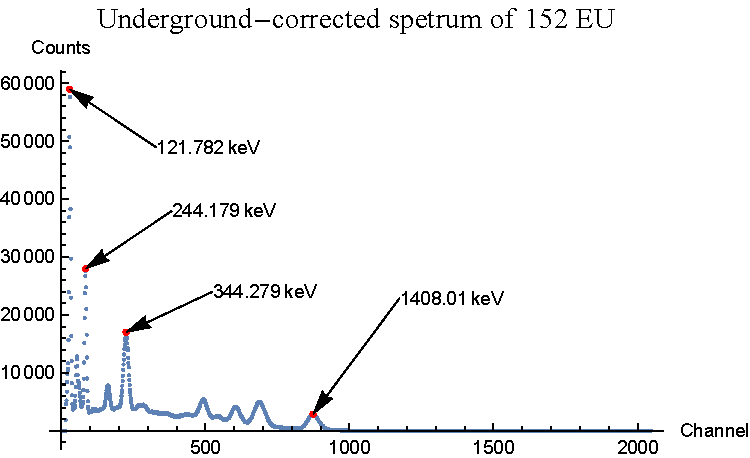
\includegraphics[scale=1.1]{EuropiumLin.pdf}
\caption{Measured spectrum of 152 EU with underground correction and used peaks marked}
\end{figure}
\newline
We use the very intense peaks for low-energy calibration, because they are very narrow, and therefore the result is very precise. But to cover a mid-ranged energy level, we use the small, but isolated peak near channel 900. The results are shown in the following table.
\begin{figure}[hbtp]
\centering
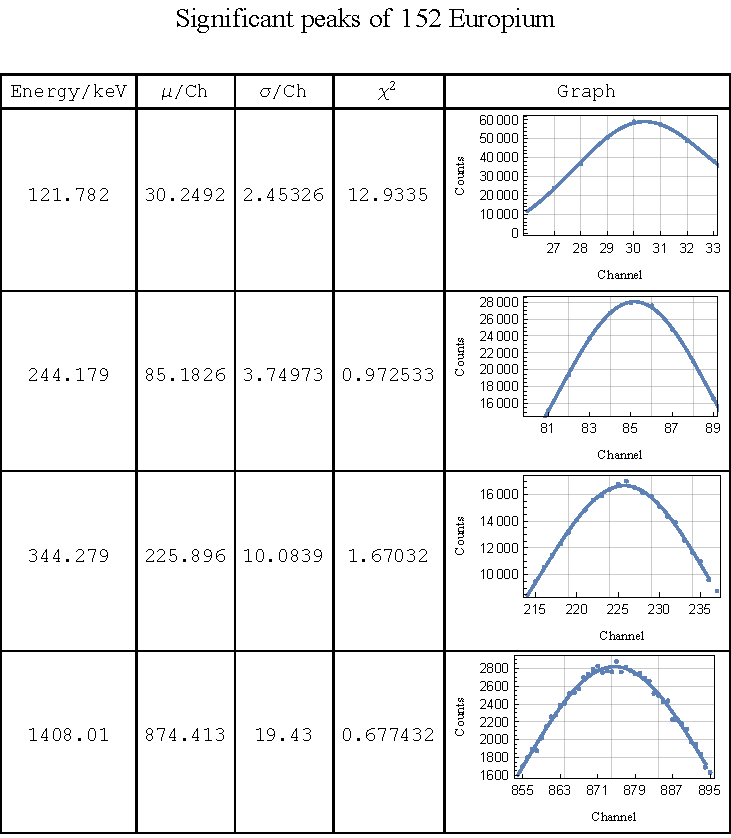
\includegraphics[scale=1.3]{EuropoiumTable.pdf}
\caption{Results of the fitting of the significant peaks of 152 EU }
\end{figure}
\newpage
Unfortunately, the first peak, which is the highest, has a high $\chi^{2}$-value. We assume this comes from the low resolution, which makes fitting difficult. The other  fits are acceptable, but because the peaks are that broad, the error for the channel-number is very high. Therefore, we have to use as many peaks as possible to get a good result. This has been made with Mathematica.

\subsection*{Natrium}
Natrium is a $\beta^{+}$-emitter. Therefore, we can detect the annihilation photons which are produced within the sample. We detect a high peak at 511 keV, and an other peak at 1274,537 keV.

\subsection*{Cobalt}
Cobalt has two significant lines, which can be used for calibration.

\subsection*{Calibrating the MCA}
Now we can use the obtained data to find a function which correlates a channel number with an energy value. We anticipate that to be a linear function. However, the properties of the MCA show, that it is better described with an s-curve, due to saturation effects. 
\begin{figure}[hbtp]
\centering
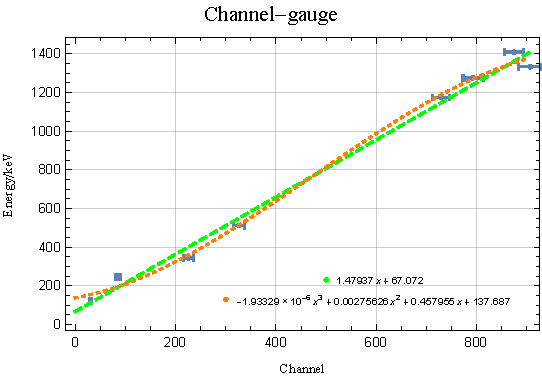
\includegraphics[scale=1.8]{Channelgauge.pdf}
\caption{Green: linear fit of the channel-energy-function; Orange: polynomial fit for the channel-energy-function}
\end{figure}
\begin{figure}[hbtp]
\centering
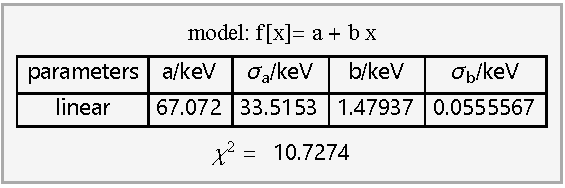
\includegraphics[scale=1]{result.pdf}
\caption{This should better be made in LaTeX directly...}
\end{figure}
We still use a linear fit, assuming that this describes the matter. The model has the form $f(x) = a + b x$. The function for the channel-energy-gauge is:
\[E[x] = ((67 \pm 34) + (1.48 \pm 0.06) x )keV\]
The $\chi^{2}$ amounts to 10.7, which is acceptable. With an amount of degrees of freedum of 6, we estimate a value of 4. With this it is possible to determine an unknown energy for a peak in the RdTh spectrum. 

As you can see, we have a huge error on the 
\end{document}